\documentclass{article}

\usepackage{graphicx}
\usepackage{tikz}
\usepackage{tikzsymbols}
\usetikzlibrary{calc,patterns,shapes.geometric}
\pagestyle{empty}
\usepackage[margin=0pt]{geometry}
\geometry{papersize={14in,12in}}

\def\centerarc[#1](#2)(#3:#4:#5){\draw[#1] ($(#2)+({#5*cos(#3)},{#5*sin(#3)})$) arc (#3:#4:#5);}

\begin{document}
	\begin{figure}
		\centering
		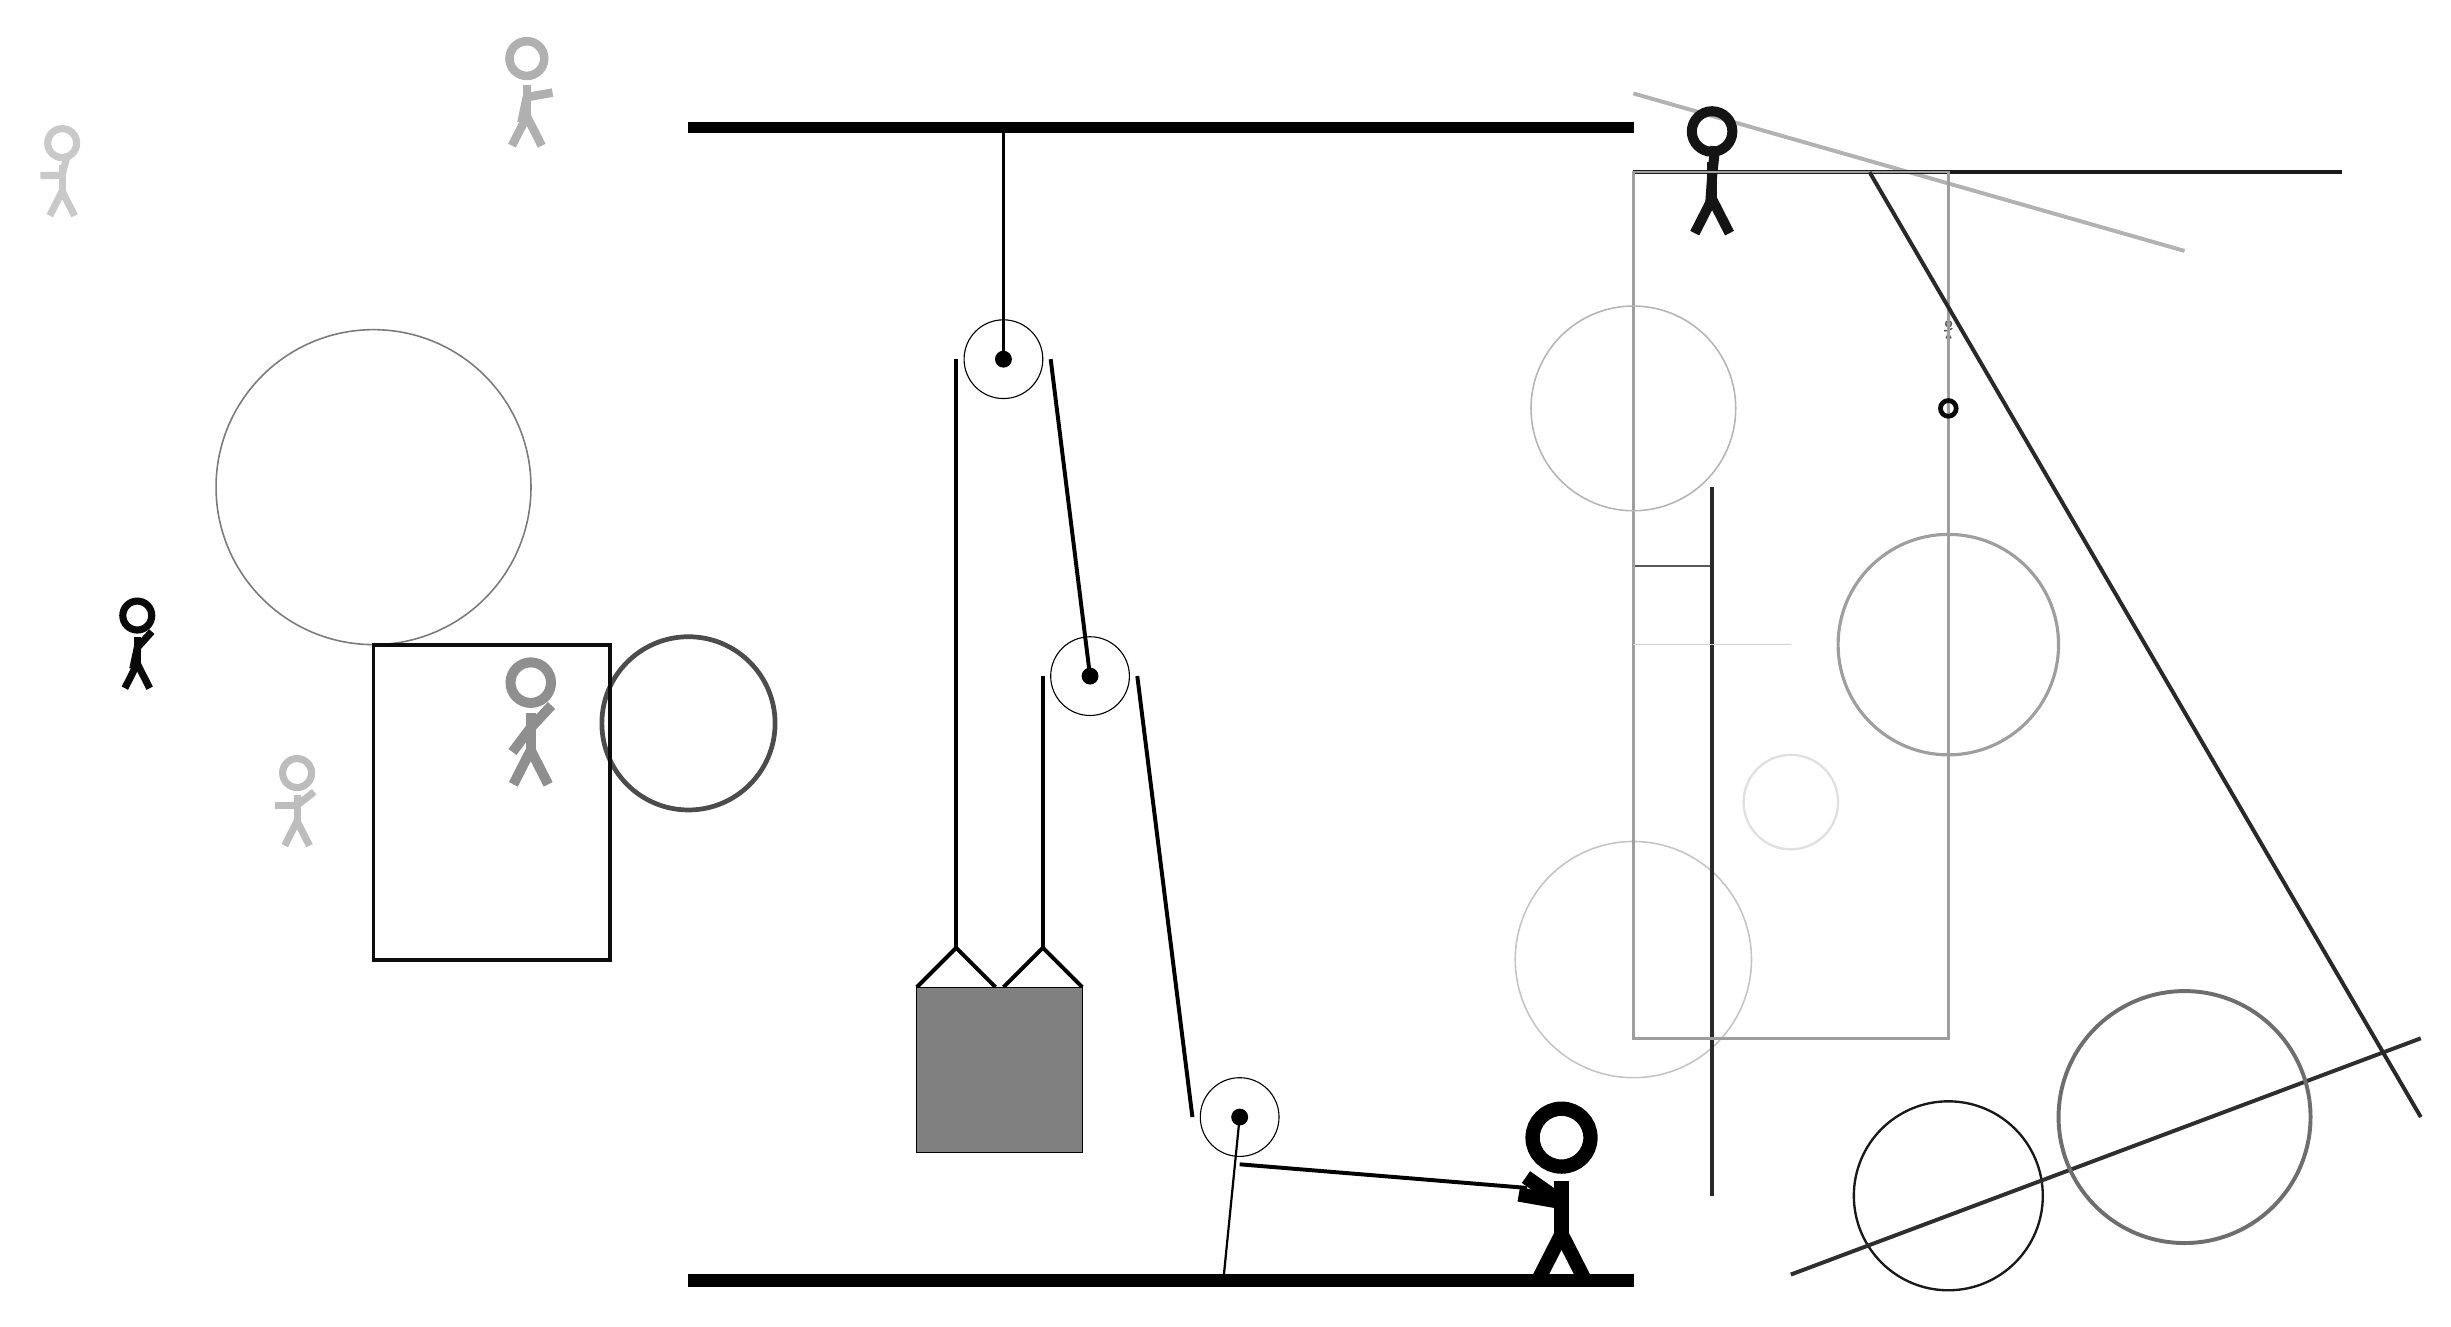
\begin{tikzpicture}
			%%%%% START %%%%%
			
			\draw[fill=black] (-2, 11.5) rectangle (10, 11.625);
			
			\node[line width=0.7mm, color=black!44] at (-4, 4) {\Strichmaxerl[7][53][47]};
			
			\draw [line width=0.3mm, color=black!90](14, -2) circle (1.2);
			\node[line width=0.2mm, color=black!21] at (-10, 11) {\Strichmaxerl[5][1][76]};
			\draw [line width=0.2mm, color=black!23](10, 1) circle (1.5);
			
			\node[line width=0.5mm, color=black!31] at (-4, 12) {\Strichmaxerl[6][78][10]};
			
			\node[line width=0.2mm, color=black!67] at (14, 9) {\Strichmaxerl[1][9][27]};
			\draw[line width=0.5mm, color=black!82](12, -3) -- (20, 0);
			\draw [line width=0.5mm, color=black!57](17, -1) circle (1.6);
			\node[line width=0.2mm, color=black!96] at (-9, 5) {\Strichmaxerl[5][78][48]};
			
			\draw[line width=0.5mm, color=black!30](10, 12) -- (17, 10);
			\draw[line width=0.5mm, color=black!89](10, 11) -- (19, 11);
			\draw [line width=0.6mm, color=black!70](-2, 4) circle (1.1);
			\node[line width=0.2mm, color=black!92] at (11, 11) {\Strichmaxerl[7][86][84]};
			
			\draw [line width=0.2mm, color=black!52](-6, 7) circle (2.0);
			\draw[line width=0.2mm, color=black!65] (11, 6) rectangle (10, 5);
			\node[line width=0.5mm, color=black!26] at (-7, 3) {\Strichmaxerl[5][0][38]};
			\draw[line width=0.5mm, color=black!95] (-3, 5) rectangle (-6, 1);
			
			\draw[line width=0.5mm, color=black!84](11, -2) -- (11, 7);
			\draw[line width=0.3mm, color=black!38] (10, 0) rectangle (14, 11);
			\draw[line width=0.2mm, color=black!18] (10, 5) rectangle (12, 5);
			\draw [line width=0.4mm, color=black!38](14, 5) circle (1.4);
			
			\draw [line width=0.6mm, color=black!96](14, 8) circle (0.1);
			\draw [line width=0.6mm, color=black!91](13, 7) circle (0.0);
			\draw [line width=0.3mm, color=black!12](12, 3) circle (0.6);
			\draw[line width=0.5mm, color=black!84](13, 11) -- (20, -1);
			
			\draw [line width=0.2mm, color=black!29](10, 8) circle (1.3);
			
			
			\draw (2, 8.625) circle (0.5);
			\draw[fill=black] (2, 8.625) circle (0.1);
			\draw[thick] (2, 8.625) -- (2, 11.5);
			
			\draw (3.1, 4.6) circle (0.5);
			\draw[fill=black] (3.1, 4.6) circle (0.1);
			
			\draw (5, -1) circle (0.5);
			\draw[fill=black] (5, -1) circle (0.1);
			\draw[thick] (5, -1) -- (4.8, -3);
			
			\draw[line width = 0.5mm]  (0.9, 0.65) -- (1.4, 1.15) -- (1.9, 0.65);
			\draw[line width = 0.5mm]  (2.0, 0.65) -- (2.5, 1.15) -- (3.0, 0.65);
			\draw[fill=black!50] (0.9, 0.65) rectangle (3.0, -1.45);
			
			\draw[line width = 0.5mm] (1.4, 8.625) -- (1.4, 1.15);
			\centerarc[line width = 0.5mm](2, 8.625)(0:180:0.6);
			\draw[line width = 0.5mm] (2.6, 8.625) -- (3.1, 4.6);
			\draw[line width = 0.5mm] (2.5, 4.6) -- (2.5, 1.15);
			\centerarc[line width = 0.5mm](3.1, 4.6)(0:180:0.6);
			\draw[line width = 0.5mm] (3.7, 4.6) -- (4.4, -1);
			\centerarc[line width = 0.5mm](5, -1)(180:270:0.6);
			\draw[line width = 0.5mm] (5, -1.6) -- (8.65, -1.9);
			
			\node at (9, -2) {\Strichmaxerl[10][-35][170]};
			
			\draw[fill=black] (-2, -3) rectangle (10, -3.15);
			
			%%%%% END %%%%%
		\end{tikzpicture}
	\end{figure}	
\end{document}